\documentclass{article}
\usepackage[utf8]{inputenc}
\usepackage{blindtext}
\usepackage{enumitem}
\usepackage{graphicx}
\usepackage{hyperref}
\usepackage{titletoc}
\graphicspath{ {images/} }

\hypersetup{colorlinks=true,
urlcolor=blue,
linkcolor=black}

\title{ \begin{center}
					
\includegraphics[scale=0.6]{../images/FEUPlogo}
				\end{center}
				\textbf{Werewolves of Miller's Hollow}}
\author{João Silva - up201405490\\
		Marcelo Ferreira - up201405323\\
		Miriam Gonçalves - up201403441}
\date{31 October, 2017}
\begin{document}

\begin{titlepage}
	\centering
	
\includegraphics[width=1\textwidth]{../images/FEUPlogo}\par\vspace{1cm}
	{\huge\bfseries Werewolves of Miller's Hollow \par}
	\vspace{2cm}
	{\scshape\Large Final Report\par}
	\vspace{1.5cm}
	{\large\bfseries Agents and Distributed Artificial Intelligence\par}
	\vspace{0.7cm}
	{\scshape\normalsize  Master in Informatics and Computing Engineering \par}
	\vspace{1.5cm}
	{\Large\itshape Group T08\textunderscore01 \par João Silva - up201405490 \par
	Marcelo Ferreira - up201405323 \par
	Miriam Gonçalves - up201403441\par}

	\vfill
% Bottom of the page
	{\large \today\par}
\end{titlepage}
\thispagestyle{empty}

\newpage

\tableofcontents

\newpage

\section{Examination Paper}
\subsection{Scenario Description}
\textit{Werewolves of Miller’s Hollow} game is based on the russian game called “Mafia” and can be played by groups between eight and eighteen people. 
Game Components (24 roles):
\begin{center}
	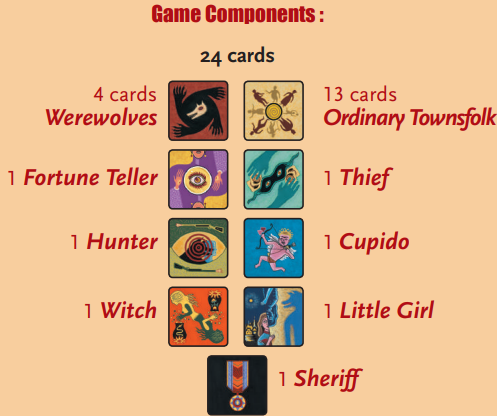
\includegraphics[scale=0.6]{../images/gamecomponents}
\end{center}
	
\begin{itemize}
	\item \textbf{4 Werewolves}; 	
	\item \textbf{13 Ordinary Townsfolk} and there are 8 different kinds of Townsperson: 
	\begin{itemize}
		\item \textbf{1 Fortune Teller} - can see the true personality of one player each night, with its capacities it will help the townsfolk to find  correctly the identity of the werewolves;
		\item \textbf{1 Thief} - if this role is used, two additional ordinary Townsfolk are added at the beginning of the game. Afterwards two cards are placed face down in the center of the table, during the preliminary turn of the first night, this player looks at these two cards and may trade his/her cards with one of them. However if both of the cards are werewolves, the Thief must trade his card with one of them. If this player takes on of the extra cards, he/she assumes the role of this player for the rest of this character for the rest of the game;
		\item \textbf{1 Hunter} - if the hunter is killed during the game he can retaliate by eliminating another player;
		\item \textbf{1 Cupido} - got the ability to make any two people fall instantly in love for the rest of the game, these two people are designated during the first night of the game. If one of the lovers die, the other must kills him/herself immediatly. In case of one of the lovers being a townsperson and the other a werewolf, they must eliminate all the other players from the game to live in love and peace;
		\item \textbf{1 Witch} - make two kind of powerful potions: one is the \textit{healing} potion that can resurrect a player killed by a werewolf, the other is a \textit{poison} that kill a player during the night. Each potion can be used only once per game and use them on him/herself;
		\item \textbf{1 Little Girl} - this character can open her eyes during the night to spy on the werewolves, but if she gets caught by them she immediatly dies instead of the designated victim;
		\item \textbf{1 Sheriff} - this role is entrusted to one of the players, this person is elected by the townsfolk and once elected this player cannot refuse the honor. Afterwards this player's votes count as two votes. If this player dies during the game he/she must name his/her successor.
	\end{itemize}
\end{itemize}

For each number of players there are different combinations of roles:
\begin{center}
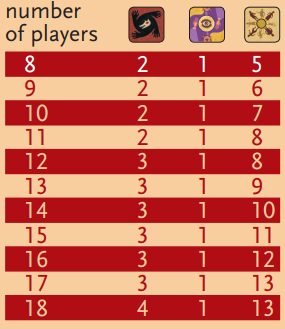
\includegraphics[scale=0.6]{../images/playermix}
\end{center}

\setlength{\parindent}{0cm}There are two phases in the game: 
\begin{itemize}
	\item the night - when werewolves devour and kill one Townsperson (that person is eliminated from the game);
	\item the day - the townsfolk try to conceal their identity and discover who the werewolves are by voting on a suspect who is eliminated from the game.	
\end{itemize}

There are several points that players need to follow for setting up the game:
\begin{itemize}
	\item the players must choose a \textit{Moderator/Narrator}, this player must know very well all the games rules and create a strong atmosphere in order for the game to be fun;
	\item the \textit{Moderator} takes the appropriate number of cards, shuffles them and deals one character card to each player, from this step the players will look at their card secretly and places it face down in front of themselves;
	\item the \textit{Narrator} puts the town to sleep, all the characters must close their eyes.
	\item depending on the character cards on play the \textit{Narrator} will call one by one and in the following order \textit{The thief}, \textit{Cupido} and \textit{The Lovers} to play their roles.
\end{itemize}
After the setting up round, the \textit{Moderator} will call \textit{The Fortune Teller} to choose a player whose true personality she wants to know, after showing her the card she will fall asleep. Next the werewolves are called to designate silently a victim which will be revealed to every players the next morning when everyone is awake.
Right after the werewolves voting for killing a person, the \textit{Moderator} will call \textit{The Witch} to wake up, show her the victim chosen and asks her if she wants to use the healing or the poisoning potion. 
The next morning, every \textit{Townsperson} will wake up, know the character/s that was/were killed during the night and will try to unmask a \textit{werewolf} without letting anyone know their true identity by voting on one player that they think that is a \textit{Werewolf}, after being eliminated from the game this player will reveal his/her identity and will not be able to speak to the other players until the game ends, while the \textit{werewolves} will try to disguise themselves as ordinary Townsfolk and not be discovered by the other players.
The game will follow these steps repeatidly until the game ends.

The game ends when:
\begin{itemize}
	\item the townsfolk manage to eliminate all the werewolves;
	\item the werewolves kill the last townsperson;
	\item the lovers are the surviving townsperson/werewolf pair, and the all other players are dead; 
\end{itemize}

\subsection{Objectives}

The purpose of our work is to create a set of agent architectures that are able to play the game. Different architectures will have different properties; Some will have act completely randomly while other will try to negotiate and argumentate to reach consensus. In the end we will evaluate and compare their performances.


\section{Specification}

\subsection{Agents Identification and Characterization}
\subsubsection{game\_coordinator agent}
This agent is what was previously called as the \textit{narrator} of the game, wil control the game flow. Responsible for switching turns during the day and night, verifying if there are enough players on game and making the right setup of the game. 
The game\_coordinator agent has the following parts:
\begin{itemize}
	\item \textbf{enough\_players} - verify if the game has enough players;
	\item \textbf{all\_werewolves\_voted} - verify if all the werewolves voted during their turn;
	\item \textbf{everyone\_has\_voted} - verify if all the players voted during the day turn;
	\item \textbf{twonsfolk\_have\_won} - verify if all the werewolves are dead;
	\item \textbf{werewolves\_have\_won} - verify if all the twonsfolk are dead;
	\item \textbf{create\_agents} - create every other type of agents in order to start a game;
	\item \textbf{setup\_game} -  do the initial setup and start the game;
	\item \textbf{inform\_fortune\_teller} - tell fortune\_teller about the other players on game;
	\item \textbf{inform\_werewolves} - tell werewolves about the other players on game;
	\item \textbf{inform\_townsfolk} - tell townsfolk about the other players on game;
	\item \textbf{start\_turn} - starts a game turn;
	\item \textbf{wake\_up\_fortune\_teller} - wake up fortune\_teller and tell her other player true personality;
	\item \textbf{wake\_up\_werewolves} - checks if there is any left townsfolk left alive and then wake up the werewolves;
	\item \textbf{voted\_to\_eliminate} - all werewolves vote and then that townsperson is killed;
	\item \textbf{wake\_up\_town} - wake up all players;
	\item \textbf{voted\_to\_lynch} - after all players voted, lynch the player with most votes;
	\item \textbf{ready} - players update their beliefs after someone being killed;
	\item \textbf{tell\_personality} - tell to the fortune\_teller the true personality of a player;
	\item \textbf{reset} - reset the game.
\end{itemize} 
\subsubsection{townsperson\_random agent}
This agent will act as a townsperson with random behaviours, it will vote randomly on other player to be lynched and has the following characteristics:
\begin{itemize}
	\item \textbf{living\_werewolves} - initial belief of how many werewolves are playing; 
	\item \textbf{player} - add others player to that townsfolk database;
	\item \textbf{day} - wake up and vote on other player randomly;
	\item \textbf{dead} - remove the dead player from the player database;
\end{itemize}

\subsubsection{townsperson\_strategic agent}
A townsperson\_strategic agent will vote based on certainty factors. 
His/her beliefs are accompanied by a certainty factor that ranges from 0 to 1. For example, if a agent believes another to be a werewolf then the belief will be represented as: 
\newline
\textbf{werewolf(player, 0.5)} 
\newline
This would be in its belief base, meaning that the agent is reasonably sure that player is a werewolf. The beliefs will be updated when:
\begin{enumerate}
	\item the player wakes up and find out who's been killed, from other player's vote the player can determine:
	\begin {enumerate}
		\item who the other players wants to see dead;
		\item if the voter wants to kill the player, then the player may suspect that the voter is a werewolf;
		\item if the voter wants to kill a player that the player thinks is a werewolf, then the player may suspect the voter is a townsperson;
		\item if the voter wants to kill a player that the player thinks is a townsperson, then the player may suspect the voter is a werewolf;
	\end{enumerate}
	\item the player finds out how the others have voted
	\begin{enumerate}
		\item if the player believes some players wanted the player who died dead, then the player may suspect that they are werewolves
	\end{enumerate}
\end{enumerate}
The beliefs must be revised every time, and past information should be taken into account in future belief updates. If the player receives contradicting information then their belief will stay the same (most likely).

This agent will act based on certainty factors created and calculated based on others players actions and has the following characteristics:
\begin{itemize}
	\item \textbf{living\_werewolves} - initial belief of how many werewolves are playing; 
	\item \textbf{player} - add others player to that townsfolk database;
	\item \textbf{day} - wake up and vote on other player that believes to be a werewolf, the one with the highest certainty werewolf factor;
	\item \textbf{voted\_to\_lynch} - updates the database beliefs taking into account other player votes and actions;
	\item \textbf{dead} - delete dead players from the player database and beliefs database.
\end{itemize}

\subsubsection{townsperson\_negotiator agent}
This agent has the following characteristics:
\begin{itemize}
	\item \textbf{living\_werewolves} - initial belief of how many werewolves are playing; 
	\item \textbf{player} - add others player to that townsfolk database;
	\item \textbf{day} - wake up and select the player that believes to be the most likely werewolf and votes on that player;
	\item \textbf{voted\_to\_lynch} - updates the database beliefs taking into account other players votes and actions;
	\item \textbf{dead} - delete dead players from the player database and beliefs database.
\end{itemize}
\subsubsection{werewolf\_random agent}
The werewolf\_random agent will vote on a townsperson randomly to die, without saving any state and votes from other players in its database. It will vote always without any knowledge of others players previous actions.
This agent has the following characteristics:
\begin{itemize}
	\item \textbf{werewolf} - add others werewolves to the player database, knowing who are the others werewolves playing;
	\item \textbf{player} - add the townsfolk players to the player database, knowing who are the enemies that are playing;
	\item \textbf{day} - wake up during the day turn and vote randomly on a townsperson;
	\item \textbf{night} - wake up during the night turn and vote randomly on a townsperson;
	\item \textbf{dead} - delete dead players from the player database,
\end{itemize}
\subsubsection{werewolf\_strategic agent}
This kind of agent will act based on townsfolk previous actions, it will try to determine which of the townsfolk knows the true identity of a werewolf and then it will vote on that player to die during the night turn.
The probability of a townsperson knowing the true identity of a werewolf will increase everytime a townsperson:
\begin{enumerate}
	\item votes on the player;
	\item votes on another werewolf;
\end{enumerate}
This agent has the following characteristics:
\begin{itemize}
	\item \textbf{alive} - initial state, the werewolf believes that is alive;
	\item \textbf{werewolf} - add others werewolves to the player database, knowing who are the others werewolves playing;
	\item \textbf{player} - add the townsfolk players to the player database, knowing who are the enemies that are playing;
	\item \textbf{night} - wake up during the night turn and votes on the townsperson that the player believes to be reasonably sure of knowing a werewolf true identity;
	\item \textbf{day} -wake up during the day turn and votes on the townsperson that the player believes to be reasonably sure of knowing a werewolf true identity;
	\item \textbf{voted\_to\_lynch} - updates the players beliefs taking into account the townsfolk votes;
	\item \textbf{dead} - deleted dead players from the player and beliefs database;
\end{itemize}
\subsubsection{werewolf\_negotiator agent}

\subsubsection{fortune\_teller agent}
\subsection{Interaction Protocols}
\section{Development}
\subsection{Platform/Tool}
\subsection{Development Environment}
\subsection{Application Structure}
\subsection{Classes Diagram}
\subsection{Implementation Details}
\section{Experiments}
\section{Enhancements}
\section{Resources}

\subsection{Software}
Eclipse \par
\url{http://www.eclipse.org/} \par
\vspace{3mm}
JADE \par
\url{http://jade.tilab.com/} \par 
\vspace{3mm}
Jason \par
\url{http://Jason.sourceforge.net/wp/} \par 

\subsection{Bibliography}
\noindent
(1) Wooldridge Michael, "An Introduction to MultiAgent Systems"

\noindent
(2) Ashraf El-Sisi, Hamdy Mousa, "Argumentation Based Negotiation in Multi-agent System"

\noindent
(3) Sarit Kraus, Katia Sycara, Amir Evenchik, "Reaching agreements through argumentation: a logical model and implementation"

\noindent
(4) Stuart Russell, Peter Norvig, "Artificial Intelligence: A Modern Approach"

\end{document}